\chapter{Résultats}
\label{ch:ch3}

Durant cet enseignement d'intégration, nous avons obtenu de nombreux résultats, en particulier en combinant différents jeux de données (global, multislice et visuel).
Dans cette partie, nous nous concentrerons sur les deux résultats principaux.

\section{Modèles}

Dans un premier temps, notre travail s'est focalisé sur deux modèles de classification : la forêt aléatoire \textit{Random Forest} et la régression logistique.

\vspace{0.3cm}

Pour assurer le bon fonctionnement de nos programmes, ces modèles s'appuient sur deux fonctions essentielles : \texttt{SMOTE} et \texttt{GroupShuffleSplit}.

\vspace{0.3cm}

\texttt{SMOTE} permet de rééquilibrer les classes dans le jeu d'entraînement.

\texttt{GroupShuffleSplit} garantit que les différentes phases d'un même patient ne soient pas séparées entre le jeu d'entraînement et le jeu de test.

\section{Résultat 1 : AUC pour le dataset global}

\begin{figure}[H]
\centering
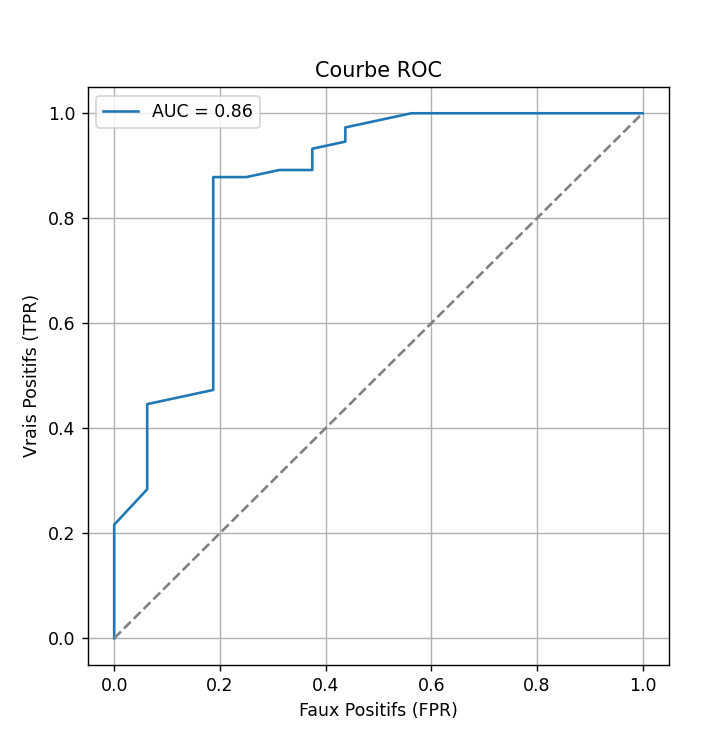
\includegraphics[width=0.3\textwidth]{img/AUC_global.png}
\caption{AUC pour le dataset global}
\label{fig:auc_global}
\end{figure}

\vspace{0.5cm}

On observe une valeur d'AUC de 0{,}84, ce qui correspond à un modèle globalement performant.